\lettrine[findent=0.4em, nindent=0em]{\textbf{P}}{robabilistic analysis} of
multiprocessor systems is an extensive and diverse area, which is expanding with
an accelerating pace. The reason for the rapid growth is that multiprocessor
systems become more sophisticated and refined, and that they penetrate deeper
into everyday life. Therefore, the impact of uncertainty inevitably becomes more
prominent and engender more severe consequences, necessitating an adequate
treatment. In order to develop efficient and reliable products, the designer has
to be equipped with tools capable of accounting for sources of uncertainty
present in multiprocessor systems.

Sources of uncertainty can be divided into analog and digital. The major
representative of the former is process variation \cite{srivastava2005}, which
has been central for many lines of research \cite{bhardwaj2008, juan2012,
lee2013, ukhov2014, ukhov2015}. Process variation is a side effect of the
fabrication process. In contrast, the sources of uncertainty labeled as
``digital'' are phenomena of the digital world rather than physical. To
elaborate, many applications running on modern devices exhibit nondeterministic
behaviors: their characteristics change from one activation to another
depending, for instance, on the runtime and input data. The digital class has
not been deprived of attention either, especially in the real-time community
\cite{diaz2002, quinton2012, tanasa2015}. Both analog and digital sources of
uncertainty render the behavior of the system at hand as essentially random, and
accounting for them is highly beneficial if not essential.

In order to account for uncertainty, one has to quantify it first. Uncertainty
quantification is a broad term, and the techniques under this generous umbrella
can deliver radically different pieces of information about the quantity of
interest. In this paper, we are interested in probability distributions rather
than, for instance, corner cases. Designing for the worst case is often a poor
solution as the system at hand might easily end up being too conservative,
over-designed \cite{quinton2012}. The value of probability distributions is well
understood, and it is especially high in the context of soft real-time systems
and control systems.

When it comes to uncertainty quantification and estimation of probability
distributions, computer experiments \cite{santner2003} are of great use.
Compared to other techniques for probabilistic analysis, computer experiments
are straightforward to undertake. The system at hand is treated as being
completely opaque, and it only needs to be simulated a number of
times---following an adequate sampling strategy---in order to draw well-grounded
conclusions about the system. Consider, for instance, the classical Monte Carlo
(\abbr{MC}) sampling, which is arguably the most famous and versatile approach
to the analysis of stochastic systems. The technique was introduced in the
middle of the twentieth century and since then has expanded into a rich family
of methods that have had a tremendous impact both in academia and in terms of
industrial breakthroughs. The success of \abbr{MC} sampling is due to the ease
of implementation, independence of the stochastic dimensionality, and asymptotic
behavior of the quantities estimated using this approach.

The major problem with sampling techniques, however, is in sampling: one should
be able to obtain sufficient many realizations of the quantity of interest in
order to be able to draw sound conclusions with respect to that quantity
\cite{diaz-emparanza2002}. The main concerns here are: How many samples do we
need? How many samples can we afford? How long does it take to obtain one
sample? How much does one sample cost? When the subject of analysis is
expensive---as measured by the metric that makes the most sense to the problem
at hand---computer experiments are rendered as slow and often infeasible.

In this paper, we propose a system-level design-time framework for the analysis
of multiprocessor systems that are dependent on uncertain parameters. The
framework can be applied in scenarios with a limited knowledge about the joint
probability distribution of the parameters, which are common in practice. Our
focal point is digital sources of uncertainty introduced earlier, which should
not be perceived as a restriction but rather as a prominent application. Similar
to \abbr{MC} methods, the framework treats the system at hand as a ``black box''
and, hence, is straightforward to apply since no handcrafting is required and
existing codes need no change. Consequently, the quantities that the framework
is able to analyze are diverse; the examples include the end-to-end delay,
energy consumption, and thermal dynamics. In contract to \abbr{MC} methods, our
technique explores the structure of the problem---that is, the dependence of the
quantity of interest on the uncertain parameters---by exercising the ``black
box'' at a set of adaptively chosen points. The adaptivity allows for reduction
of the costs associated with the system's evaluation. The magnitude of reduction
depends on the problem, and it can be substantial when the problem is well
disposed to adaptation. Furthermore, the output of the proposed framework is
generative: we construct a light representation of the quantity of interest that
can be used to generate realizations of this quantity without touching the
original expensive ``black box.'' Consequently, given the representation, all
the computer-experiments machinery applies and costs practically nothing.

\begin{figure}
  \centering
  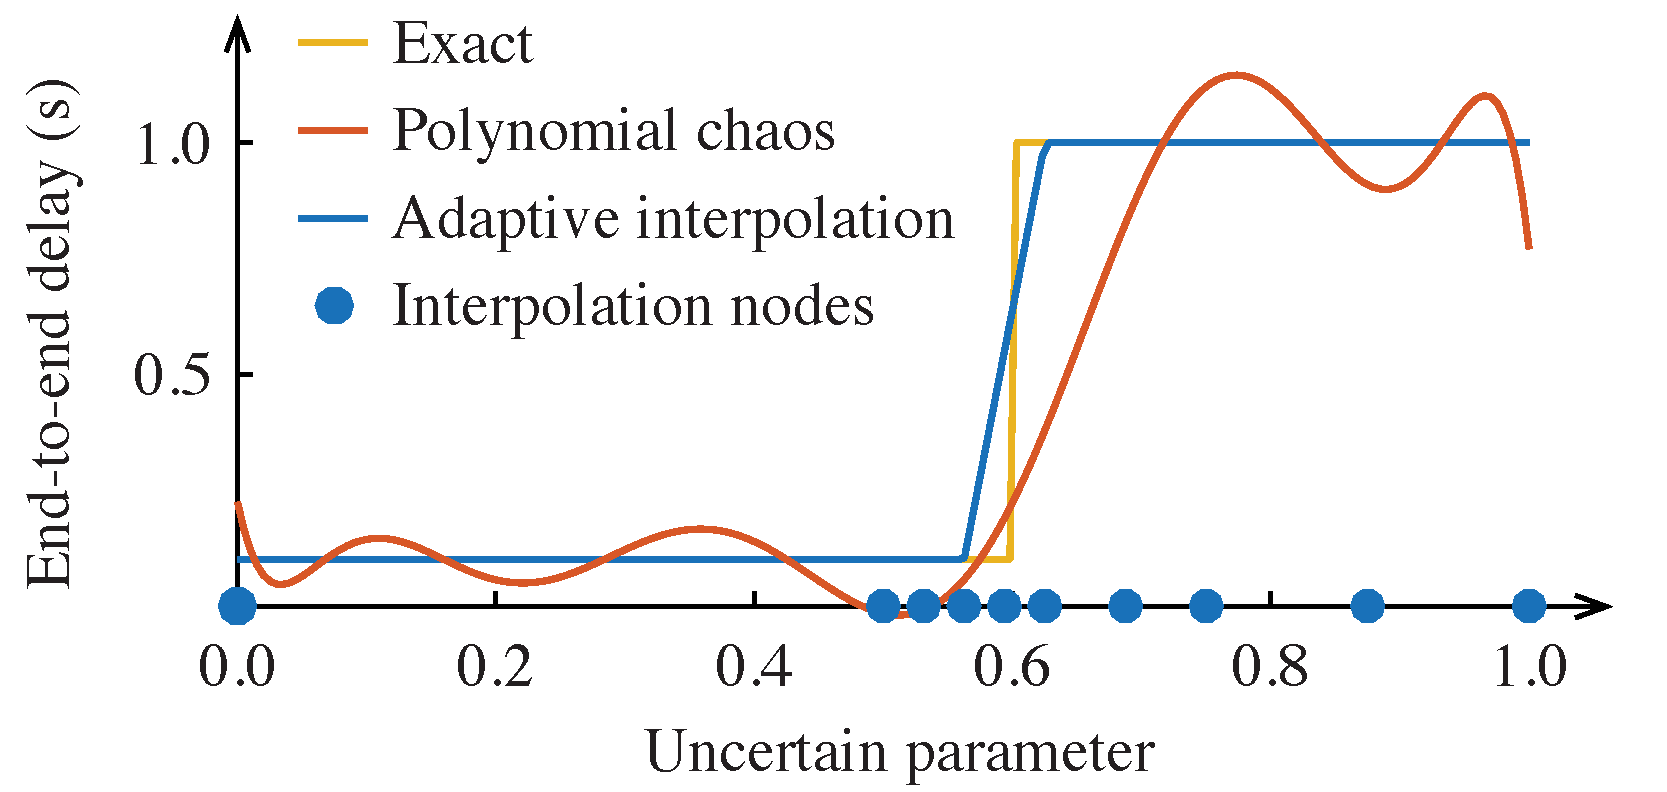
\includegraphics[width=1.0\columnwidth]{include/assets/figures/motivation.pdf}
  \caption{
    A motivational example.
  }
  \flab{motivation}
\end{figure}

The approach that we take belongs to the class of stochastic collocation
techniques \cite{xiu2010}. The major distinctive feature of stochastic
collocation is the usage of interpolation as a means of uncertainty
quantification, which should be contrasted with other techniques such as
polynomial-chaos (\abbr{PC}) expansions relying on regression. The application
of \abbr{PC} expansions is limited in this case due to the non-smoothness of the
response surface. More concretely, our framework is based on adaptive
hierarchical interpolation on sparse grids \cite{klimke2006, ma2009}.

The remainder of the paper is organized as follows. Section~\ref{sec:prior-work}
provides an overview of the prior work. In \sref{present-work}, we summarize the
contribution of the present paper. The preliminaries are given in
\sref{preliminaries}. The objective of our study is formulated in
\sref{problem-formulation}. The proposed framework is presented in
\sref{modeling}, \sref{interpolation}, and \sref{analysis}. The experimental
results are reported and discussed in \sref{experimental-results}, and
\sref{conclusion} concludes the paper.
